\documentclass[9pt,twocolumn,twoside]{styles/osajnl}
\usepackage{fancyvrb}
\journal{i524} 

\title{Microsoft Azure Data Factory}

\author[1]{Sowmya Ravi}

\affil[1]{School of Informatics and Computing, Bloomington, IN 47408, U.S.A.}


\affil[*]{Corresponding authors: laszewski@gmail.com}

\dates{project-000, \today}

\ociscodes{Cloud, Data, Movement, Transformaion}

% replace this with your url in github/gitlab
\doi{\url{https://github.com/sowravi}}


\begin{abstract}
Azure Data Factory is a cloud based data integration service that handles and automates data movement and data integration services. The Data Factory stands out in its ability to ingest data from multiple sources, efficiently build pipelines to manage processes and visualize the results in a pragmatic manner. This paper discusses the data movement and data transformation activities supported by Azure Data Factory \newline
\end{abstract}

\setboolean{displaycopyright}{true}

\begin{document}

\maketitle

\section{Introduction}
The cloud based data integration service is designed to pull data from various sources, transform/ process data and publish the result to the data stores. A data management gateway enables access to data on SQL Databases~\cite{www-jamesserra}. The data processing is done by It works by creating pipelines to  transform the raw data into a format that can be readily used by BI Tools or applications. The services comes with rich visualization aids that aid data analysis. Data Factory supports two types of activities: data movement  and data transformation. Data Movement~\cite{www-microsoft-azure} is a Copy Activity in Data Factory that copies data from a data source to a Data sink. Data Factory supports the following data stores. Data from any source can be written to any sink.  Data Transformation:  Azure Data Factory supports the following transformation activities such as Map reduce, Hive transformations and Machine learning activities.
Data factory is a great tool to analyze web data, sensor data and geo-spatial data.	
\begin{figure}[htbp]
\centering
\fbox{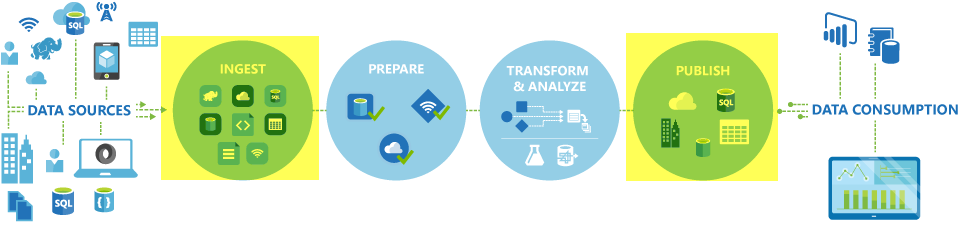
\includegraphics[width=\linewidth]{images/azure-data.png}}
\caption{Work flow in Azure Data Factory}
\label{fig:copy-local}
\end{figure}


\section{Datasets in Azure Data Factory}

The JSON format is used to store data in Azure Data Factory~\cite{www-microsoft-azure-data}.In Azure data factory creating a dataset essentially means creating a pointer to the data to be processed.
The data store could be tables, files, folders, and documents. After a dataset is created, it can be used with activities in a pipeline which will be discussed later in the paper. For example, a dataset can be an input/output dataset of a Copy Activity or an HDInsightHive Activity. A visual layout of all your pipelines and data inputs and outputs is also provided by Azure. It enables one all the relationships and dependencies of  pipelines across all sources. Thus, it is possible to keep track of all data sources and sinks.

\section{Pipelines and Activities in Azure Data Factory}
\subsection{Data Pipeline}
Azure Data Factory used pipelines to organize work flow and data processing.~\cite{www-microsoft-azure-pipelines} A pipeline is an ordering of processes in accordance with the logic relation existing between the processes. 

\subsection{Activity} 
An activity is a process or action that is taken on the data.~\cite{www-microsoft-azure-pipelines} An activity takes zero or more datasets as inputs and produces zero or more datasets as an output. The activities are grouped under data movement of data transformation activities.

\subsubsection{Data Movement}
The Data Movement is achieved by the Data Factory copy wizard. Data can be copied either from local or cloud sources with ease for further transformation to be carried out. The copy activity is highly secure, reliable and scalable

When the source as well as the sink data stores are in the cloud, Copy Activity goes through the following stages to copy data. 
\begin{itemize}
    \item Reads data from the source data store\item Performs serialization/de-serialization, compression/decompression, column mapping, and type conversion. It does these operations based on the configurations of the input dataset, output dataset, and Copy Activity.\item Writes data to the destination data store
\end{itemize}

In case of moving a data located on-premises to cloud, data management gateway must be installed in the local machine containing the data.The data management gateway is required to perform e serialization/de-serialization, compression/decompression, column mapping, and type conversion. The data management gateway directly writes the data to the destination. The following figure shows the copy activity from a local machine
\begin{figure}[htbp]
\centering
\fbox{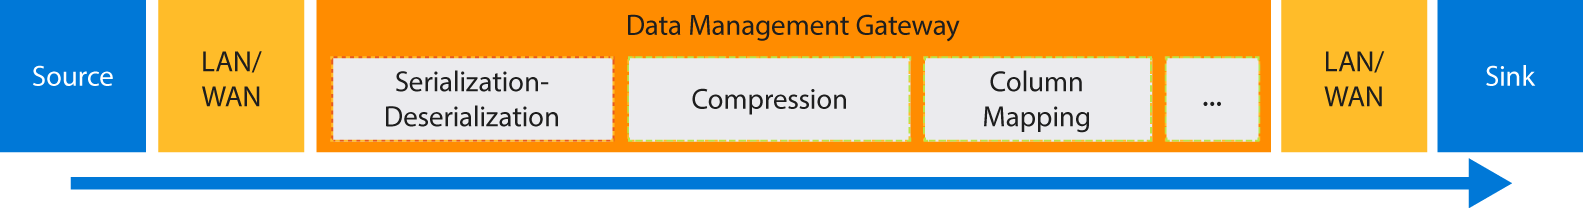
\includegraphics[width=\linewidth]{images/copy2.png}}
\caption{Moving data between on-premises and cloud data stores}
\label{fig:copy-local}
\end{figure}

The Azure Data Factory is connected to a variety of data stores and supports different data formats~\cite{www-microsoft-azure-copy}. Copy Activity also reads from and writes to files in specified formats: text, Avro, ORC, Parquet, and JSON, and compression codec GZip, Deflate, BZip2, and ZipDeflate are supported. Furthermore,~\cite{www-microsoft-azure-copy} pipelines could be created either using the copy wizard or using the JSON scripts. The scheduling facility make it possible to run multiple copy operations one after the other in a sequential manner. After copying, the data is ready for transformation purpose

\subsubsection{Data Transformation}

Data transformation activities transform the raw data to derive predictions and insights. 
The Data Factory comes with two types of computing environments
\begin{itemize}
    \item On Demand: This type of environment is solely managed by Data Factory. The environment is created before a process begins and is automatically removed when the process is completed
    \item: Bring your own: An individual can register his/her computing environment and has to be managed by the individual.
\end{itemize}

The following transformations are supported By Azure Data Factory~\cite{www-microsoft-azure-transform}
\begin{itemize}
    \item HDInsight Hive activity: The HDInsight Hive activity executes Hive queries on your own or on-demand Windows/Linux-based HDInsight cluster.~\cite{www-microsoft-azure-hive}
    \item HDInsight Pig activity: The HDInsight Pig activity in a Data Factory pipeline executes Pig queries on your own or on-demand Windows/Linux-based HDInsight cluster.~\cite{www-microsoft-azure-pig}
    \item HDInsight MapReduce activity: The HDInsight MapReduce activity in a Data Factory pipeline executes MapReduce programs on your own or on-demand Windows/Linux-based HDInsight cluster.~\cite{www-microsoft-azure-map}
    \item HDInsight Streaming activity: HDInsightStreamingActivity Activity is used to invoke a Hadoop Streaming job from an Azure Data Factory pipeline. The HDInsight Streaming Activity in a Data Factory pipeline executes Hadoop Streaming programs on your own or on-demand Windows/Linux-based HDInsight cluster.~\cite{www-microsoft-azure-hsa}
    \item Machine Learning activities: Azure Data Factory helps in building and deploying predictive models in the following three steps.~\cite{www-microsoft-azure-ml}
    \begin{enumerate}
        \item Create a training experiment: This is done using the Azure ML Studio. The ML studio is a collaborative visual development environment that can be used to train and test a predictive analytics model using training data.
        \item Convert it to a predictive experiment: Once the model has been trained with existing data, it can be used to score new data, prepare and streamline the experiment for scoring.
        \item Deploy it as a web service. The experiment can be published using an Azure web service. 
    \end{enumerate}
    \item Stored procedure activity: A procedure that is already stored can be invoked in one of the following data stores:  Azure SQL Database, Azure SQL Data Warehouse, SQL Server Database in your enterprise or on an Azure virtual machine (VM).~\cite{www-microsoft-azure-stored} 
    \item Data Lake Analytics U-SQL activity: Azure Data Lake Analytics can be linked to the compute service in the Data Factory. ~\cite{www-microsoft-azure-datalake}
    \item .NET custom activity: One can create an activity with a customized logic to be used in a pipeline ~\cite{www-microsoft-azure-dotnet}
\end{itemize}

\section{Monitoring and Management}
The Data Factory has a monitor and manage app which helps keep tab of available resources, handle alerts and monitor various views. The resource explorer has a tree view and a diagram view of all the existing pipelines, datasets and linked services. ~\cite{www-microsoft-azure-moniter}

\section{Use Cases}
Data factory can be used for a wide range of applications such as Product recommendations, Customer profiling etc. The sample solution for a recommendation system is illustrated in Fig.3.
\begin{figure}[htbp]
\centering
\fbox{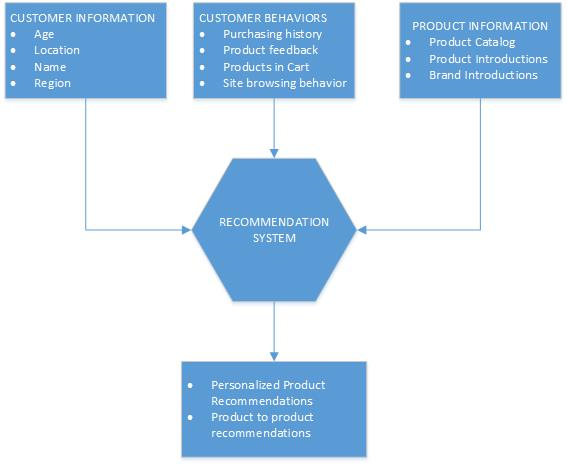
\includegraphics[width=\linewidth]{images/reco.png}}
\caption{A recommendation engine using Azure Data factory}
\label{fig:copy-local}
\end{figure}
In this case, the customer information, product information and the behavioural data of the customer are stored in azure blobs. The combined data is fed to the recommendation system which is modelled using any of the algorithms available in the Azure Machine Learning suite. The final result contains customer specific product recommendations that can be written to relational database for the consumption by the store's website.

\section{Conclusion}
The paper talks about the data orchestration and management using Microsoft's Data Factory. It's ability to link diverse data stores makes it a versatile tool for data integration. In addition, the powerful pipeline based data transformation services embedded in it helps data scientists and developers to provide efficient and effective solutions using large datasets. 

% Bibliography

\bibliography{references}
 
\section*{Author Biographies}
\begingroup
\setlength\intextsep{0pt}
\begin{minipage}[t][3.2cm][t]{1.0\columnwidth} % Adjust height [3.2cm] as required for separation of bio photos.
  \begin{wrapfigure}{L}{0.25\columnwidth}
    
\includegraphics[width=0.25\columnwidth]{images/john_smith.eps}
  \end{wrapfigure}
  \noindent
  {\bfseries Sowmya Ravi} pursuing Master's in Data Science at Indiana University, Bloomington. Her research interests include Machine learning, Data Mining and Big Data
\end{minipage}

\endgroup

\newpage

\appendix

\section{Work Breakdown}

The work on this project was distributed as follows between the
authors:

\begin{description}

\item[John Smith.] Explored the deep mathematical knowledge needed for
  this paper and taught it to the other authors.

\item[Alice Smith.] She explored the world of Oz and was instrumental
  to work on the deployment of hadoop.

\item[Bruce Wayne.] He did not contribute at all to this paper and
  flew around to safe the world.  

\end{description}

\section{Report Checklist}

\begin{itemize}
\renewcommand{\labelitemi}{\scriptsize$\square$} 
\item Have you written the report in word or LaTeX in the specified
  format?
\item Have you included the report in github/lab?
\item Have you specified the names and e-mails of all team members in
  your report. E.g. the username in Canvas?
\item Have you included the HID of all team members?
\item Does the report have the project number added to it?
\item Have you included all images in native and PDF format in gitlab
  in the images folder?
\item Have you added the bibliography file in bibtex format?
\item Have you submitted an additional page that describes who did
  what in the project or report?
\item Have you spellchecked the paper?
\item Have you made sure you do not plagiarize?
\item Have you made sure that the important directories are all lower
  case and have no underscore or space in it?
\item Have you made sure that all authors have a README.rst in their
  HID github/lab repository?
\item Have you made sure that there is a README.rst in the project
  directory and that it is properly filled out?
\item Have you put a work breakdown in the document if you worked in a
  group?
\end{itemize}

\end{document}
